\documentclass{article}
\usepackage{amsmath}
\usepackage{graphicx}

\begin{document}


\section*{A) (2 points)}
If you create a main() routine that calls \texttt{fork()} twice, i.e. if it includes the following code:
\begin{verbatim}
pid_t x=-11, y=-22;
x = fork();
if(x>0) y = fork();
\end{verbatim}
Assuming all \texttt{fork()} calls succeed, draw a process tree similar to that of Fig. 3.8 (page 116) in your textbook, clearly indicating the values of x and y for each process in the tree (i.e. whether 0, -11, -22, or larger than 0).
Note that the process tree should only have one node for each process and thus the number of nodes should be equal to the number of processes.
The process tree should be a snapshot just after all forks completed but before any process exists.
Each line/arrow in the process tree diagram shall represent a creation of a process, or alternatively a parent/child relationship.




\section*{B) (4 points)}
Write a program that creates the process tree shown below:

\begin{center}
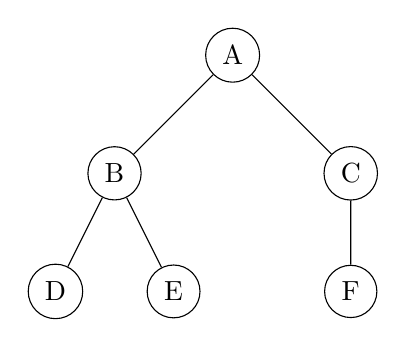
\begin{tikzpicture}[level distance=1.5cm,
  level 1/.style={sibling distance=3cm},
  level 2/.style={sibling distance=1.5cm}]
  \node [circle, draw] {A}
    child {node [circle, draw] {B}
      child {node [circle, draw] {D}}
      child {node [circle, draw] {E}}
    }
    child {node [circle, draw] {C}
      child {node [circle, draw] {F}}
    };
\end{tikzpicture}
\end{center}
Each node represents a process, and the edges represent the parent-child relationship.  Process A is the initial process.  Your program should use \texttt{fork()} appropriately.  Clearly label each process in your code with its corresponding letter from the tree.





\section*{C) (4 points)}
Write a program whose main routine obtains two parameters, a and b, from the user (i.e., passed to your program when it was invoked from the shell, a and b are integers greater than 0).  The main process then creates a child process. The child process calculates the greatest common divisor (GCD) of a and b using Euclid's algorithm and prints the result.  The parent process waits for the child to finish and then prints the least common multiple (LCM) of a and b, calculated using the formula LCM(a, b) = (a * b) / GCD(a, b). Do not use IPC in your solution to this problem (i.e. neither shared memory nor message passing).  You can assume the inputs will always result in a valid LCM calculation (no division by zero).




\end{document}